\documentclass{article}
\usepackage{graphicx}
\usepackage{tocloft} 
\usepackage{glossaries}
\usepackage{lipsum}
\usepackage{geometry}
\usepackage{fancyhdr} 
\usepackage{amsmath}
\usepackage{biblatex}  
\geometry{a4paper, margin=1in}

\title{User Manual}
\author{Group 1 }
\date{\today}

\begin{document}
\maketitle  
\pagebreak

\tableofcontents
\pagebreak


\includegraphics[width=0.3\linewidth]{../logo/csula.png} 

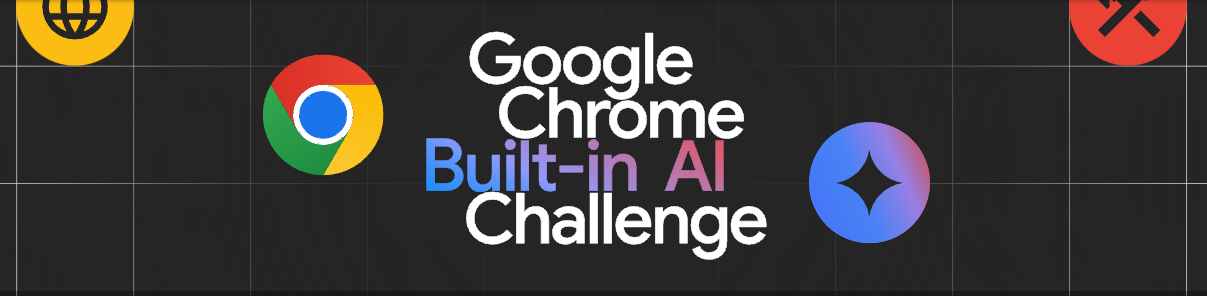
\includegraphics[width=0.3\linewidth]{../logo/chromeai.png} 
\section{Introduction}
\subsection{Purpose}
This document serves as a guide with clear instructions on how to install, access, and utilize the application. It's designed to help users understand the main functionalities, troubleshoot common issues, and make the most of the AI-driven tools.

\subsection{Intended Audience}
This manual is intended for any user who wants to simplify their research, communication, and writing tasks with the help of AI.

\subsection{Goals and Reasons}
The application reduces manual effort in summarizing large texts, ensures quick translations, improves writing quality, and provides dynamic prompts for enhanced productivity.

\section{System Requirements}
\begin{itemize}
    \item \textbf{Browser:} Google Chrome (version 100 or later).
    \item \textbf{Platform:} Works on Windows, macOS, Linux, and ChromeOS.
    \item \textbf{Internet Connection:} Required only for initial installation and future updates, but afterward the AI runs locally and doesn't require a connection.
\end{itemize}

\section{Installation \& Access}
\subsection{Web Application}
\begin{enumerate}
    \item Visit the hosted URL: \url{https://aplplicationpage.com}
    \item Click the "Sign Up" button if you are a new user to create an account or click "Log In" if you already have an account.
    \item Once logged in, you will see the main dashboard.
\end{enumerate}

\subsection{Chrome Extension}
\begin{enumerate}
    \item Open the Chrome Web Store and search for "AI Enhanced Browser Tool".
    \item Click "Add to Chrome".
    \item Once installed, the extension icon will appear next to your address bar.
\end{enumerate}

\section{Navigating the Interface}
The main dashboard provides access to:
\begin{itemize}
    \item \textbf{Prompt Input Field:} Enter queries or instructions to interact with the AI.
    \item \textbf{Summarization Tool:} Paste or upload text to get a concise summary.
    \item \textbf{Translation Panel:} Select the language you want and input text to translate.
    \item \textbf{Rewrite Suggestions:} Paste text to receive alternative wordings.
\end{itemize}

\section{Using the Features}
\subsection{Prompt Generation}
\begin{enumerate}
    \item Click on the "Prompts" tab.
    \item Type your query (e.g., "Generate a summary of this article: ...").
    \item Press "Enter" and the AI will provide an immediate suggestion.
\end{enumerate}

\subsection{Summarization}
\begin{enumerate}
    \item Click on the "Summarize" tab.
    \item Paste or upload the text and click "Summarize".
    \item The output panel will show a summary below the original text.
\end{enumerate}

\subsection{Translation}
\begin{enumerate}
    \item Click on the  "Translate" tab.
    \item Select the source (if not automatically detected) and target languages from the dropdown menus.
    \item Type or paste your text and click "Translate".
    \item The translated text appears immediately.
\end{enumerate}

\subsection{Rewriting Text}
\begin{enumerate}
    \item Click on the "Rewrite" tab.
    \item Paste your text and select "Rewrite".
    \item Choose from the suggested alternatives that appear on the right panel.
\end{enumerate}

\section{Troubleshooting \& FAQs}
\begin{itemize}
    \item \textbf{No AI response:} Check if Chrome or the App is up-to-date or restart the browser.
    \item \textbf{Language not recognized:} Manually select both source and target languages before translating.
\end{itemize}

\section{Contact \& Support}
For additional support or feedback, please visit our GitHub repository’s issue page at \url{https://github.com/saulc/Cs3338-final-project.git}  where you'll find multiple ways to contact us.
\end{document}